\appendix
\chapter{Appendix}

\section{Dataset}

\begin{center}
	\scriptsize
	\captionof{table}{Number of dataset rows per asset}
	\label{tab:appendix_dataset_rows}
	\vspace{0.5em}
	\resizebox{1\textwidth}{!}{%
		{\renewcommand{\arraystretch}{1.2}
			\begin{tabular}{llr}
				\hline
				Category & Asset & Dataset Rows \\
				\hline
				Blue-chip Stocks & Ayala Corporation & 3,235 \\
				Blue-chip Stocks & Jollibee Foods Corporation & 3,234 \\
				Blue-chip Stocks & SM Investments Corporation & 3,233 \\
				\hline
				Penny Stocks & Araneta Properties & 2,956 \\
				Penny Stocks & PH Resorts Group & 2,680 \\
				Penny Stocks & United Paragon Mining Corporation & 2,240 \\
				\hline
				Cryptocurrency & Bitcoin & 4,848 \\
				Cryptocurrency & Litecoin & 3,283 \\
				Cryptocurrency & XRP & 3,627 \\
	
				\hline
			\end{tabular}
		}
	}
\end{center}
Table~\ref{tab:appendix_dataset_rows} shows the number of dataset rows for each asset included in the study. The dataset sizes are not the same across all assets. Bitcoin has the largest dataset, while United Paragon Mining Corporation has the smallest.


\section{Experiment 1 Tables}
\label{app:experiment1_tables}


\begin{center}
	\scriptsize
	\captionof{table}{Validation performance of blue-chip stocks}
	\label{tab:val_bluechip}
	\vspace{0.5em}
	\resizebox{\textwidth}{!}{%
		{\renewcommand{\arraystretch}{1.3}
			\begin{tabular}{lllccccc}
				\hline
				Stock & Model & Metric & CHV-SKF & EW-WFV & NWFV & BCV & BCV-PU \\
				\hline
				Ayala Corporation & CNN--TIC & Accuracy & 68.19\% & 71.79\% & 73.32\% & 67.87\% & 70.07\% \\
				& CNN--TIC & Macro F1 & 51.56\% & 58.49\% & 58.31\% & 52.65\% & 52.39\% \\
				& CNN--MIC & Accuracy & 65.33\% & 72.08\% & 71.72\% & 66.80\% & 66.91\% \\
				& CNN--MIC & Macro F1 & 49.69\% & 57.22\% & 57.02\% & 51.51\% & 49.55\% \\
				\hline
				Jollibee Food Corporation & CNN--TIC & Accuracy & 67.86\% & 64.86\% & 66.28\% & 60.56\% & 69.50\% \\
				& CNN--TIC & Macro F1 & 51.69\% & 49.57\% & 50.91\% & 45.88\% & 47.49\% \\
				& CNN--MIC & Accuracy & 67.29\% & 69.39\% & 68.16\% & 64.07\% & 68.26\% \\
				& CNN--MIC & Macro F1 & 51.38\% & 51.28\% & 52.72\% & 46.46\% & 46.73\% \\
				\hline
				SM Investments & CNN--TIC & Accuracy & 72.85\% & 75.40\% & 76.91\% & 70.52\% & 78.89\% \\
				& CNN--TIC & Macro F1 & 55.31\% & 63.52\% & 63.74\% & 56.60\% & 59.55\% \\
				& CNN--MIC & Accuracy & 73.66\% & 74.03\% & 75.92\% & 72.05\% & 74.68\% \\
				& CNN--MIC & Macro F1 & 55.94\% & 61.65\% & 63.27\% & 56.92\% & 57.69\% \\
				\hline
			\end{tabular}
	}}
\end{center}

\begin{center}
	\scriptsize
	\captionof{table}{Validation performance of penny stocks}
	\label{tab:val_penny}
	\vspace{0.5em}
	\resizebox{\textwidth}{!}{%
		{\renewcommand{\arraystretch}{1.3}
			\begin{tabular}{lllccccc}
				\hline
				Stock & Model & Metric & CHV-SKF & EW-WFV & NWFV & BCV & BCV-PU \\
				\hline
				United Paragon Mining & CNN--TIC & Accuracy & 67.17\% & 70.37\% & 73.04\% & 67.50\% & 66.77\% \\
				& CNN--TIC & Macro F1 & 54.35\% & 56.38\% & 58.03\% & 52.14\% & 50.75\% \\
				& CNN--MIC & Accuracy & 62.60\% & 69.21\% & 71.11\% & 67.30\% & 68.91\% \\
				& CNN--MIC & Macro F1 & 50.97\% & 55.98\% & 57.25\% & 50.66\% & 50.36\% \\
				\hline
				PH Resorts Group & CNN--TIC & Accuracy & 73.11\% & 70.53\% & 75.00\% & 68.58\% & 69.97\% \\
				& CNN--TIC & Macro F1 & 52.41\% & 56.45\% & 57.83\% & 49.35\% & 45.48\% \\
				& CNN--MIC & Accuracy & 70.84\% & 69.55\% & 71.39\% & 66.89\% & 63.79\% \\
				& CNN--MIC & Macro F1 & 50.36\% & 56.80\% & 57.21\% & 48.84\% & 46.35\% \\
				\hline
				Araneta Properties & CNN--TIC & Accuracy & 70.20\% & 72.90\% & 72.80\% & 73.60\% & 72.94\% \\
				& CNN--TIC & Macro F1 & 51.92\% & 61.92\% & 62.37\% & 58.45\% & 57.75\% \\
				& CNN--MIC & Accuracy & 70.09\% & 72.75\% & 70.83\% & 73.06\% & 73.84\% \\
				& CNN--MIC & Macro F1 & 52.12\% & 64.02\% & 60.66\% & 57.61\% & 56.74\% \\
				\hline
			\end{tabular}
	}}
\end{center}

\begin{center}
	\scriptsize
	\captionof{table}{Validation performance of cryptocurrencies}
	\label{tab:val_crypto}
	\vspace{0.5em}
	\resizebox{\textwidth}{!}{%
		{\renewcommand{\arraystretch}{1.3}
			\begin{tabular}{lllccccc}
				\hline
				Stock & Model & Metric & CHV-SKF & EW-WFV & NWFV & BCV & BCV-PU \\
				\hline
				Bitcoin & CNN--TIC & Accuracy & 67.71\% & 66.33\% & 67.81\% & 69.47\% & 67.59\% \\
				& CNN--TIC & Macro F1 & 48.83\% & 53.64\% & 55.16\% & 48.01\% & 47.58\% \\
				& CNN--MIC & Accuracy & 66.79\% & 67.26\% & 67.92\% & 66.88\% & 68.42\% \\
				& CNN--MIC & Macro F1 & 47.61\% & 55.04\% & 54.76\% & 47.09\% & 48.61\% \\
				\hline
				Litecoin & CNN--TIC & Accuracy & 70.27\% & 68.89\% & 71.87\% & 69.44\% & 66.09\% \\
				& CNN--TIC & Macro F1 & 54.85\% & 54.85\% & 55.11\% & 51.50\% & 48.34\% \\
				& CNN--MIC & Accuracy & 72.53\% & 72.73\% & 72.95\% & 66.81\% & 63.37\% \\
				& CNN--MIC & Macro F1 & 54.98\% & 56.61\% & 55.77\% & 49.62\% & 45.98\% \\
				\hline
				XRP & CNN--TIC & Accuracy & 73.04\% & 73.33\% & 73.96\% & 70.41\% & 67.95\% \\
				& CNN--TIC & Macro F1 & 54.82\% & 56.11\% & 57.67\% & 52.68\% & 50.81\% \\
				& CNN--MIC & Accuracy & 72.83\% & 70.49\% & 71.41\% & 70.89\% & 63.89\% \\
				& CNN--MIC & Macro F1 & 53.65\% & 54.98\% & 55.91\% & 52.43\% & 47.64\% \\
				\hline
			\end{tabular}
	}}
\end{center}

\section{Experiment 2 Tables}
\label{app:experiment2_tables}
\begin{center}
	\scriptsize
	\captionof{table}{Test classification performance of blue-chip stocks}
	\label{tab:test_bluechip}
	\vspace{0.5em}
	\resizebox{\textwidth}{!}{%
		{\renewcommand{\arraystretch}{1.3}
			\begin{tabular}{lllccccc}
				\hline
				Stock & Model & Metric & CHV-SKF & EW-WFV & NWFV & BCV & BCV-PU \\
				\hline
				Ayala Corporation & CNN--TIC & Accuracy & 69.24\% & 67.55\% & 67.55\% & 74.22\% & 65.84\% \\
				& CNN--TIC & Macro F1 & 52.43\% & 51.36\% & 51.36\% & 51.24\% & 49.72\% \\
				& CNN--MIC & Accuracy & 64.76\% & 63.04\% & 63.04\% & 65.68\% & 68.63\% \\
				& CNN--MIC & Macro F1 & 49.26\% & 49.02\% & 49.02\% & 50.51\% & 52.36\% \\
				\hline
				Jollibee Food Corp. & CNN--TIC & Accuracy & 67.02\% & 68.90\% & 68.90\% & 78.38\% & 70.30\% \\
				& CNN--TIC & Macro F1 & 51.66\% & 54.37\% & 54.37\% & 52.85\% & 52.77\% \\
				& CNN--MIC & Accuracy & 68.34\% & 69.05\% & 69.05\% & 73.09\% & 72.78\% \\
				& CNN--MIC & Macro F1 & 48.41\% & 53.07\% & 53.07\% & 56.27\% & 51.74\% \\
				\hline
				SM Investments & CNN--TIC & Accuracy & 70.98\% & 64.54\% & 64.54\% & 70.14\% & 83.51\% \\
				& CNN--TIC & Macro F1 & 54.28\% & 49.09\% & 49.09\% & 50.99\% & 55.35\% \\
				& CNN--MIC & Accuracy & 69.39\% & 46.81\% & 46.81\% & 65.79\% & 79.00\% \\
				& CNN--MIC & Macro F1 & 51.36\% & 39.54\% & 39.54\% & 49.82\% & 57.03\% \\
				\hline
			\end{tabular}
	}}
\end{center}

\begin{center}
	\scriptsize
	\captionof{table}{Test classification performance of penny stocks}
	\label{tab:test_penny}
	\vspace{0.5em}
	\resizebox{\textwidth}{!}{%
		{\renewcommand{\arraystretch}{1.3}
			\begin{tabular}{lllccccc}
				\hline
				Stock & Model & Metric & CHV-SKF & EW-WFV & NWFV & BCV & BCV-PU \\
				\hline
				United Paragon Mining & CNN--TIC & Accuracy & 69.21\% & 68.52\% & 68.52\% & 70.82\% & 69.18\% \\
				& CNN--TIC & Macro F1 & 53.67\% & 57.74\% & 57.74\% & 59.58\% & 55.69\% \\
				& CNN--MIC & Accuracy & 73.73\% & 66.89\% & 66.89\% & 69.51\% & 56.72\% \\
				& CNN--MIC & Macro F1 & 51.11\% & 54.20\% & 54.20\% & 59.49\% & 50.54\% \\
				\hline
				PH Resorts Group & CNN--TIC & Accuracy & 59.37\% & 70.76\% & 70.76\% & 75.89\% & 75.27\% \\
				& CNN--TIC & Macro F1 & 46.99\% & 50.72\% & 50.72\% & 51.35\% & 35.99\% \\
				& CNN--MIC & Accuracy & 65.88\% & 70.92\% & 70.92\% & 35.77\% & 40.90\% \\
				& CNN--MIC & Macro F1 & 47.84\% & 54.04\% & 54.04\% & 25.57\% & 28.47\% \\
				\hline
				Araneta Properties & CNN--TIC & Accuracy & 67.20\% & 68.73\% & 68.73\% & 66.35\% & 50.48\% \\
				& CNN--TIC & Macro F1 & 50.85\% & 49.61\% & 49.61\% & 48.38\% & 40.69\% \\
				& CNN--MIC & Accuracy & 67.58\% & 63.33\% & 63.33\% & 46.98\% & 45.08\% \\
				& CNN--MIC & Macro F1 & 50.61\% & 49.41\% & 49.41\% & 39.96\% & 36.49\% \\
				\hline
			\end{tabular}
	}}
\end{center}

\begin{center}
	\scriptsize
	\captionof{table}{Test classification performance of cryptocurrencies}
	\label{tab:test_crypto}
	\vspace{0.5em}
	\resizebox{\textwidth}{!}{%
		{\renewcommand{\arraystretch}{1.3}
			\begin{tabular}{lllccccc}
				\hline
				Stock & Model & Metric & CHV-SKF & EW-WFV & NWFV & BCV & BCV-PU \\
				\hline
				Bitcoin & CNN--TIC & Accuracy & 53.25\% & 68.71\% & 68.71\% & 73.08\% & 75.99\% \\
				& CNN--TIC & Macro F1 & 32.94\% & 48.12\% & 48.12\% & 40.16\% & 39.19\% \\
				& CNN--MIC & Accuracy & 84.75\% & 51.87\% & 51.87\% & 41.68\% & 70.58\% \\
				& CNN--MIC & Macro F1 & 37.47\% & 39.89\% & 39.89\% & 27.77\% & 40.49\% \\
				\hline
				Litecoin & CNN--TIC & Accuracy & 64.66\% & 69.13\% & 69.13\% & 67.88\% & 75.88\% \\
				& CNN--TIC & Macro F1 & 49.69\% & 53.45\% & 53.45\% & 48.24\% & 54.84\% \\
				& CNN--MIC & Accuracy & 76.12\% & 75.99\% & 75.99\% & 80.98\% & 78.79\% \\
				& CNN--MIC & Macro F1 & 51.15\% & 54.31\% & 54.31\% & 52.71\% & 53.83\% \\
				\hline
				XRP & CNN--TIC & Accuracy & 69.25\% & 59.31\% & 59.31\% & 75.13\% & 58.58\% \\
				& CNN--TIC & Macro F1 & 47.90\% & 42.79\% & 42.79\% & 47.43\% & 44.40\% \\
				& CNN--MIC & Accuracy & 67.53\% & 50.16\% & 50.16\% & 65.04\% & 57.02\% \\
				& CNN--MIC & Macro F1 & 44.58\% & 31.80\% & 31.80\% & 45.47\% & 36.28\% \\
				\hline
			\end{tabular}
	}}
\end{center}

\begin{center}
	\scriptsize
	\captionof{table}{Financial performance of blue-chip stocks}
	\label{tab:fin_bluechip}
	\vspace{0.5em}
	\resizebox{\textwidth}{!}{%
		{\renewcommand{\arraystretch}{1.3}
			\begin{tabular}{lllccccc}
				\hline
				Stock & Model & Metric & CHV-SKF & EW-WFV & NWFV & BCV & BCV-PU \\
				\hline
				Ayala Corporation & CNN--TIC & Final Equity & 17,384.65 & 9,233.18 & 9,233.18 & 15,851.34 & 11,100.64 \\
				& CNN--TIC & Mean Return & 11.32\% & -3.21\% & -3.21\% & 16.06\% & 2.22\% \\
				& CNN--TIC & Std Return & 12.78\% & 13.64\% & 13.64\% & 18.95\% & 7.93\% \\
				& CNN--MIC & Final Equity & 21,715.91 & 12,314.28 & 12,314.28 & 9,853.95 & 13,770.70 \\
				& CNN--MIC & Mean Return & 16.55\% & 6.24\% & 6.24\% & -1.17\% & 10.78\% \\
				& CNN--MIC & Std Return & 15.37\% & 11.57\% & 11.57\% & 13.12\% & 19.82\% \\
				\hline
				Jollibee Food Corporation & CNN--TIC & Final Equity & 12,194.60 & 11,734.50 & 11,734.50 & 11,443.29 & 10,258.05 \\
				& CNN--TIC & Mean Return & 4.18\% & 6.27\% & 6.27\% & 5.30\% & 1.19\% \\
				& CNN--TIC & Std Return & 12.00\% & 15.70\% & 15.70\% & 14.59\% & 10.25\% \\
				& CNN--MIC & Final Equity & 11,750.14 & 15,167.17 & 15,167.17 & 12,025.72 & 10,577.82 \\
				& CNN--MIC & Mean Return & 3.34\% & 15.31\% & 15.31\% & 6.64\% & 3.66\% \\
				& CNN--MIC & Std Return & 11.54\% & 12.05\% & 12.05\% & 9.72\% & 23.78\% \\
				\hline
				SM Investments & CNN--TIC & Final Equity & 31,374.99 & 10,958.34 & 10,958.34 & 12,047.73 & 12,832.53 \\
				& CNN--TIC & Mean Return & 26.68\% & 3.28\% & 3.28\% & 6.60\% & 8.90\% \\
				& CNN--TIC & Std Return & 16.06\% & 8.64\% & 8.64\% & 9.43\% & 12.50\% \\
				& CNN--MIC & Final Equity & 25,299.63 & 8,768.61 & 8,768.61 & 9,058.43 & 13,229.06 \\
				& CNN--MIC & Mean Return & 21.14\% & -4.14\% & -4.14\% & -2.93\% & 9.61\% \\
				& CNN--MIC & Std Return & 17.79\% & 6.94\% & 6.94\% & 10.21\% & 4.83\% \\
				\hline
			\end{tabular}
	}}
\end{center}

\begin{center}
	\scriptsize
	\captionof{table}{Financial performance of penny stocks}
	\label{tab:fin_penny}
	\vspace{0.5em}
	\resizebox{\textwidth}{!}{%
		{\renewcommand{\arraystretch}{1.3}
			\begin{tabular}{lllccccc}
				\hline
				Stock & Model & Metric & CHV-SKF & EW-WFV & NWFV & BCV & BCV-PU \\
				\hline
				United Paragon Mining & CNN--TIC & Final Equity & 60,090.92 & 69,285.79 & 69,285.79 & 71,290.94 & 30,109.73 \\
				& CNN--TIC & Mean Return & 47.92\% & 93.55\% & 93.55\% & 96.47\% & 46.83\% \\
				& CNN--TIC & Std Return & 38.02\% & 41.47\% & 41.47\% & 49.26\% & 31.99\% \\
				& CNN--MIC & Final Equity & 14,362.47 & 38,171.64 & 38,171.64 & 113,842.99 & 96,526.61 \\
				& CNN--MIC & Mean Return & 8.72\% & 56.82\% & 56.82\% & 128.47\% & 116.22\% \\
				& CNN--MIC & Std Return & 16.94\% & 14.08\% & 14.08\% & 46.91\% & 45.78\% \\
				\hline
				PH Resorts Group & CNN--TIC & Final Equity & -14.45 & 9,717.88 & 9,717.88 & 11,711.74 & 5,270.44 \\
				& CNN--TIC & Mean Return & -45.36\% & -2.59\% & -2.59\% & 4.08\% & -20.66\% \\
				& CNN--TIC & Std Return & 39.91\% & 12.26\% & 12.26\% & 19.06\% & 13.29\% \\
				& CNN--MIC & Final Equity & 15,862.02 & 12,307.15 & 12,307.15 & 10,036.61 & 12,087.63 \\
				& CNN--MIC & Mean Return & 9.84\% & 5.22\% & 5.22\% & -1.41\% & 4.68\% \\
				& CNN--MIC & Std Return & 23.85\% & 13.46\% & 13.46\% & 17.35\% & 17.30\% \\
				\hline
				Araneta Properties & CNN--TIC & Final Equity & 29,615.25 & 3,803.51 & 3,803.51 & 6,039.79 & 4,109.71 \\
				& CNN--TIC & Mean Return & 28.39\% & -26.63\% & -26.63\% & -15.91\% & -24.98\% \\
				& CNN--TIC & Std Return & 40.83\% & 15.09\% & 15.09\% & 10.77\% & 18.92\% \\
				& CNN--MIC & Final Equity & 8,232.65 & 3,322.04 & 3,322.04 & 3,493.10 & 4,089.15 \\
				& CNN--MIC & Mean Return & -1.25\% & -29.82\% & -29.82\% & -29.09\% & -25.06\% \\
				& CNN--MIC & Std Return & 24.51\% & 17.65\% & 17.65\% & 14.78\% & 17.50\% \\
				\hline
			\end{tabular}
	}}
\end{center}

\begin{center}
	\scriptsize
	\captionof{table}{Financial performance of cryptocurrencies}
	\label{tab:fin_crypto}
	\vspace{0.5em}
	\resizebox{\textwidth}{!}{%
		{\renewcommand{\arraystretch}{1.3}
			\begin{tabular}{lllccccc}
				\hline
				Stock & Model & Metric & CHV-SKF & EW-WFV & NWFV & BCV & BCV-PU \\
				\hline
				Bitcoin & CNN--TIC & Final Equity & 14,336.98 & 20,817.61 & 20,817.61 & 10,969.38 & 10,754.24 \\
				& CNN--TIC & Mean Return & 7.97\% & 27.52\% & 27.52\% & 3.23\% & 2.51\% \\
				& CNN--TIC & Std Return & 11.89\% & 23.75\% & 23.75\% & 5.60\% & 4.35\% \\
				& CNN--MIC & Final Equity & 12,403.82 & 15,098.19 & 15,098.19 & 10,726.47 & 14,334.69 \\
				& CNN--MIC & Mean Return & 4.57\% & 16.12\% & 16.12\% & 2.42\% & 12.12\% \\
				& CNN--MIC & Std Return & 6.74\% & 21.74\% & 21.74\% & 4.19\% & 18.98\% \\
				\hline
				Litecoin & CNN--TIC & Final Equity & 536,049.38 & 63,289.88 & 63,289.88 & 28,289.69 & 79,559.77 \\
				& CNN--TIC & Mean Return & 125.60\% & 94.77\% & 94.77\% & 40.45\% & 101.89\% \\
				& CNN--TIC & Std Return & 54.55\% & 76.82\% & 76.82\% & 18.58\% & 37.17\% \\
				& CNN--MIC & Final Equity & 115,957.47 & 41,510.23 & 41,510.23 & 51,165.71 & 71,350.18 \\
				& CNN--MIC & Mean Return & 73.42\% & 69.62\% & 69.62\% & 79.53\% & 95.51\% \\
				& CNN--MIC & Std Return & 71.28\% & 69.80\% & 69.80\% & 64.99\% & 43.17\% \\
				\hline
				XRP & CNN--TIC & Final Equity & 47,955.76 & 11,766.81 & 11,766.81 & 13,240.01 & 19,706.72 \\
				& CNN--TIC & Mean Return & 42.99\% & 5.71\% & 5.71\% & 10.19\% & 28.84\% \\
				& CNN--TIC & Std Return & 53.71\% & 6.71\% & 6.71\% & 11.28\% & 36.62\% \\
				& CNN--MIC & Final Equity & 40,523.64 & 9,844.92 & 9,844.92 & 13,530.27 & 10,550.73 \\
				& CNN--MIC & Mean Return & 45.02\% & -0.48\% & -0.48\% & 11.40\% & 2.12\% \\
				& CNN--MIC & Std Return & 79.94\% & 3.22\% & 3.22\% & 14.54\% & 6.87\% \\
				\hline
			\end{tabular}
	}}
\end{center}

\section{Experiment 3 Class Importance}
\label{app:experiment3_shap}

This section presents the predicted-class SHAP row importance plots for the selected assets under BCV-PU. The plots show the mean absolute SHAP contribution of each technical and macroeconomic row to the predicted class. Technical indicators are shown in blue, while macroeconomic indicators are shown in red.

\begin{center}
	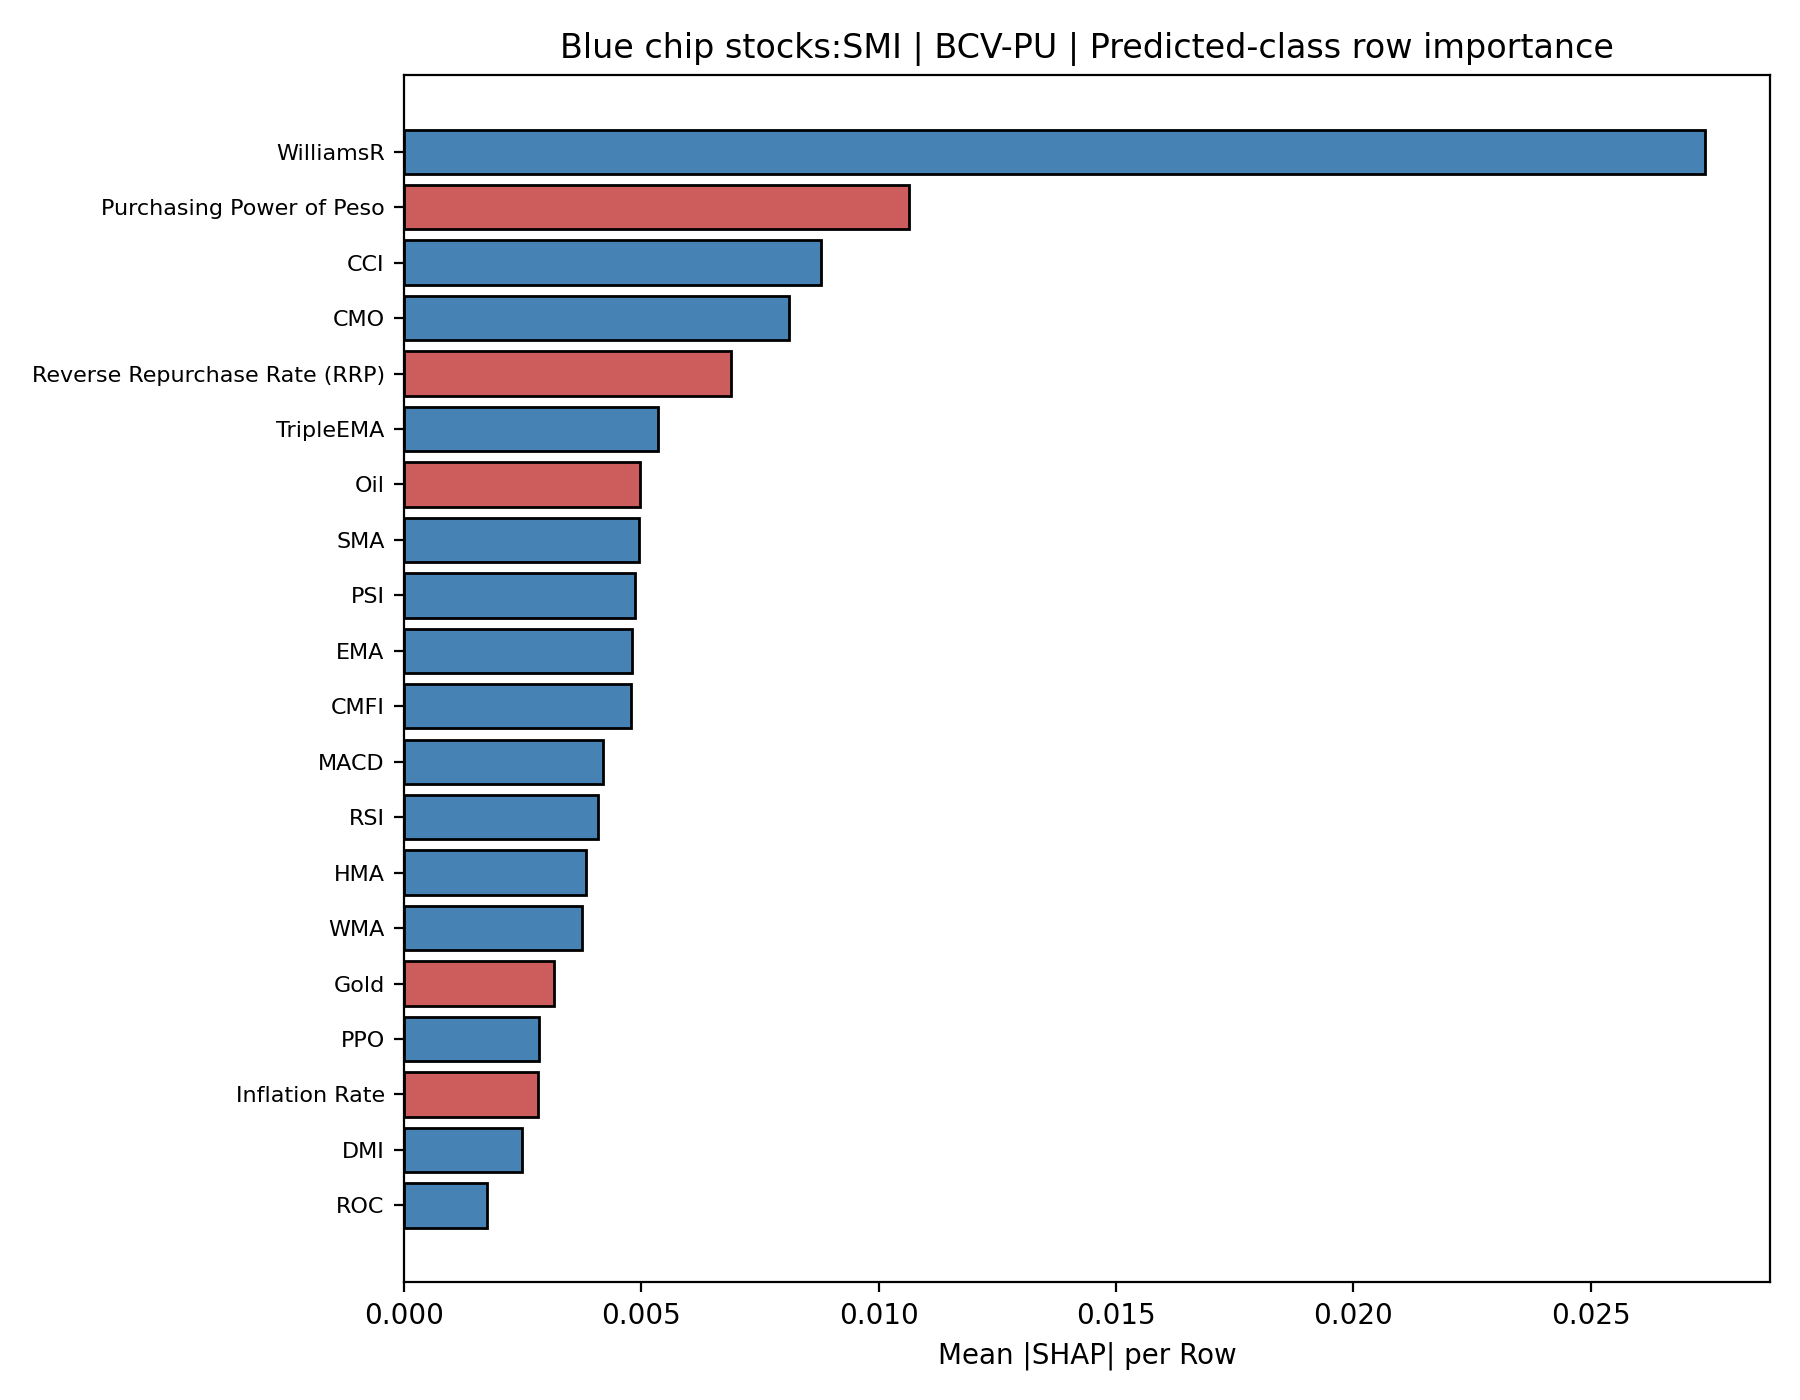
\includegraphics[width=0.32\textwidth]{../figures/SMI_PredictedClassRowImportance.png}
	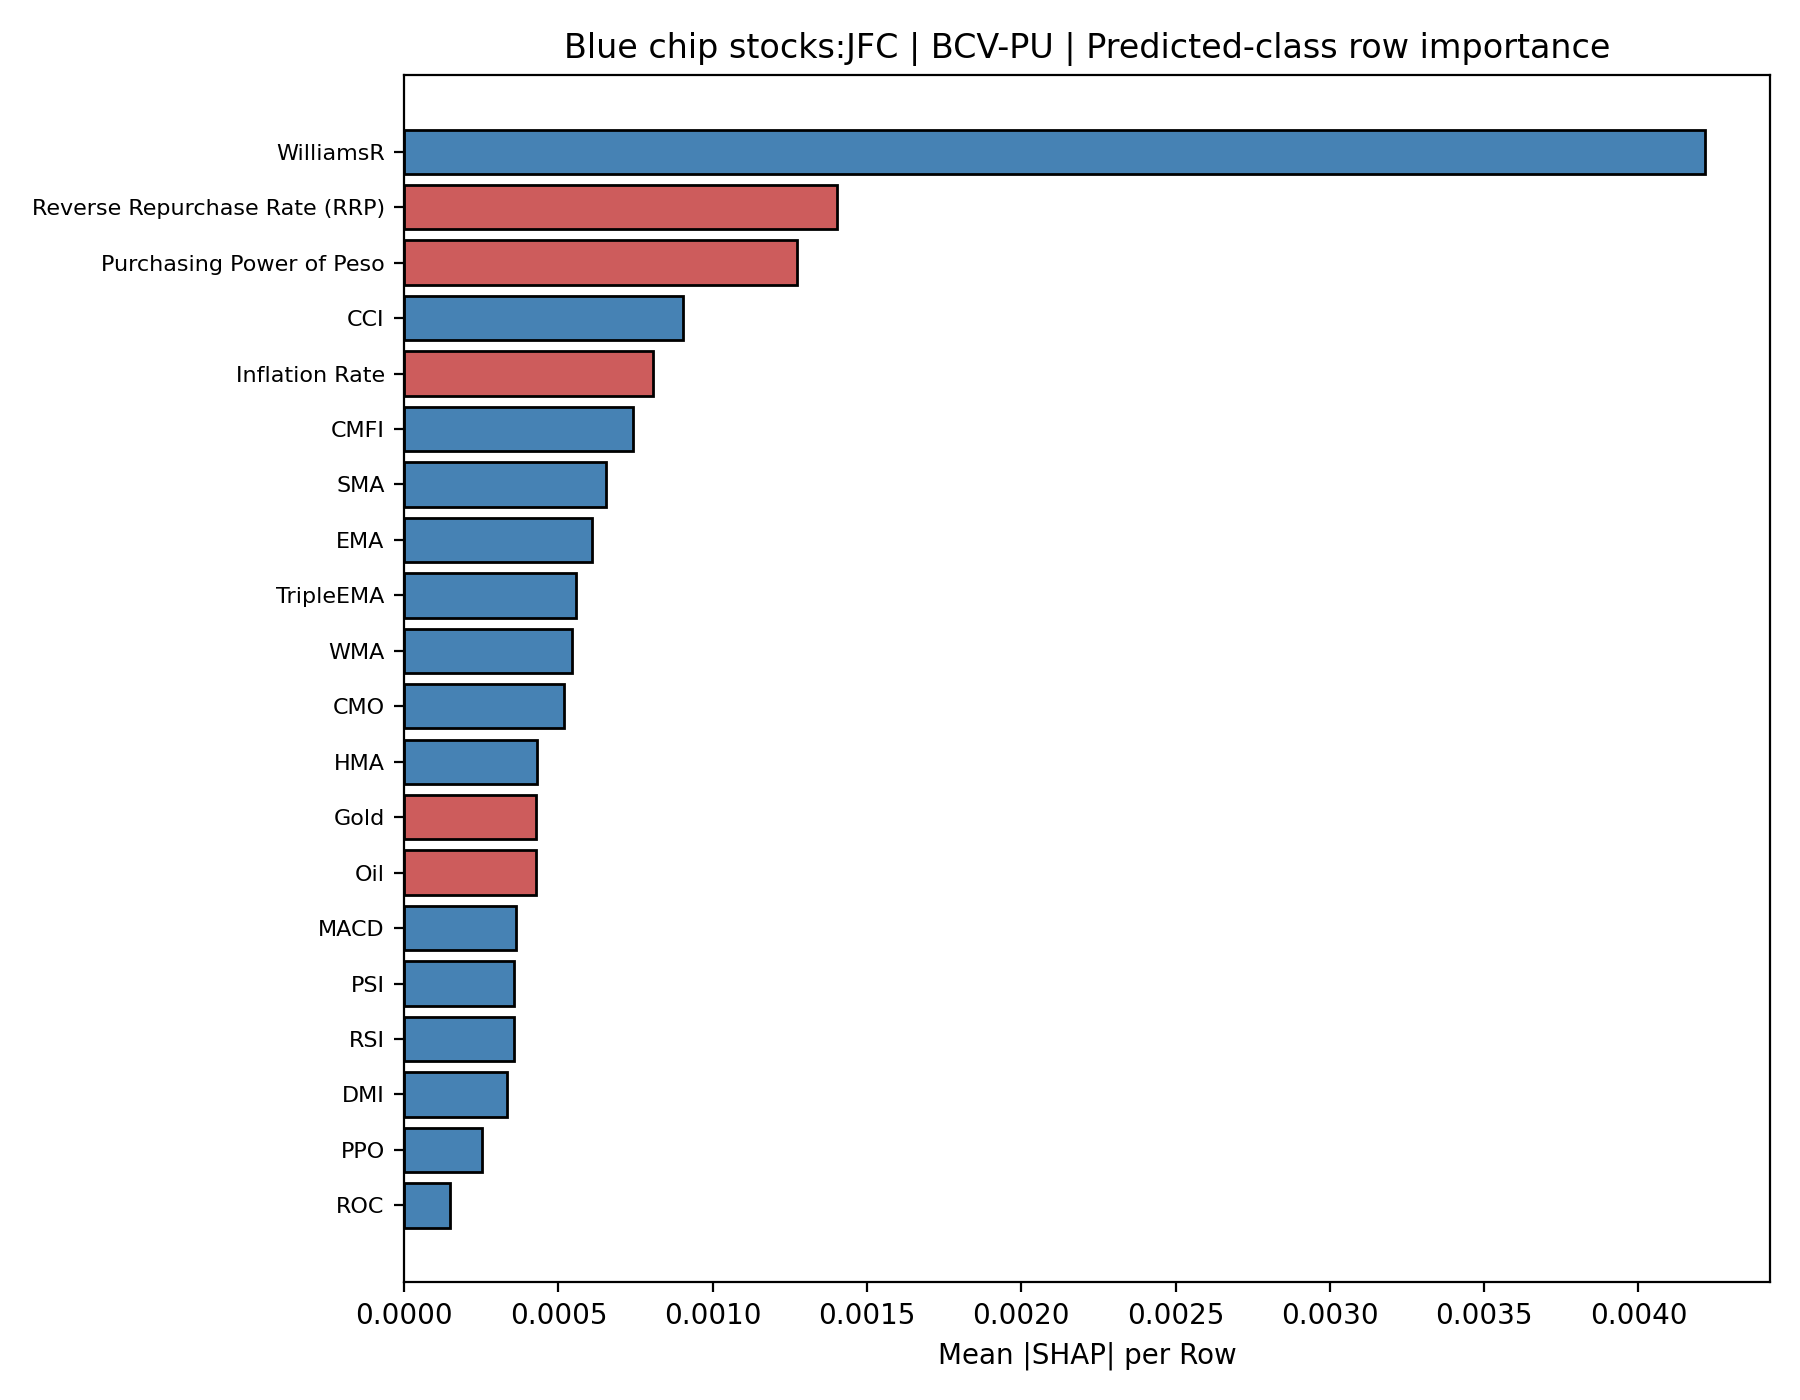
\includegraphics[width=0.32\textwidth]{../figures/JFC_PredictedClassRowImportance.png}
	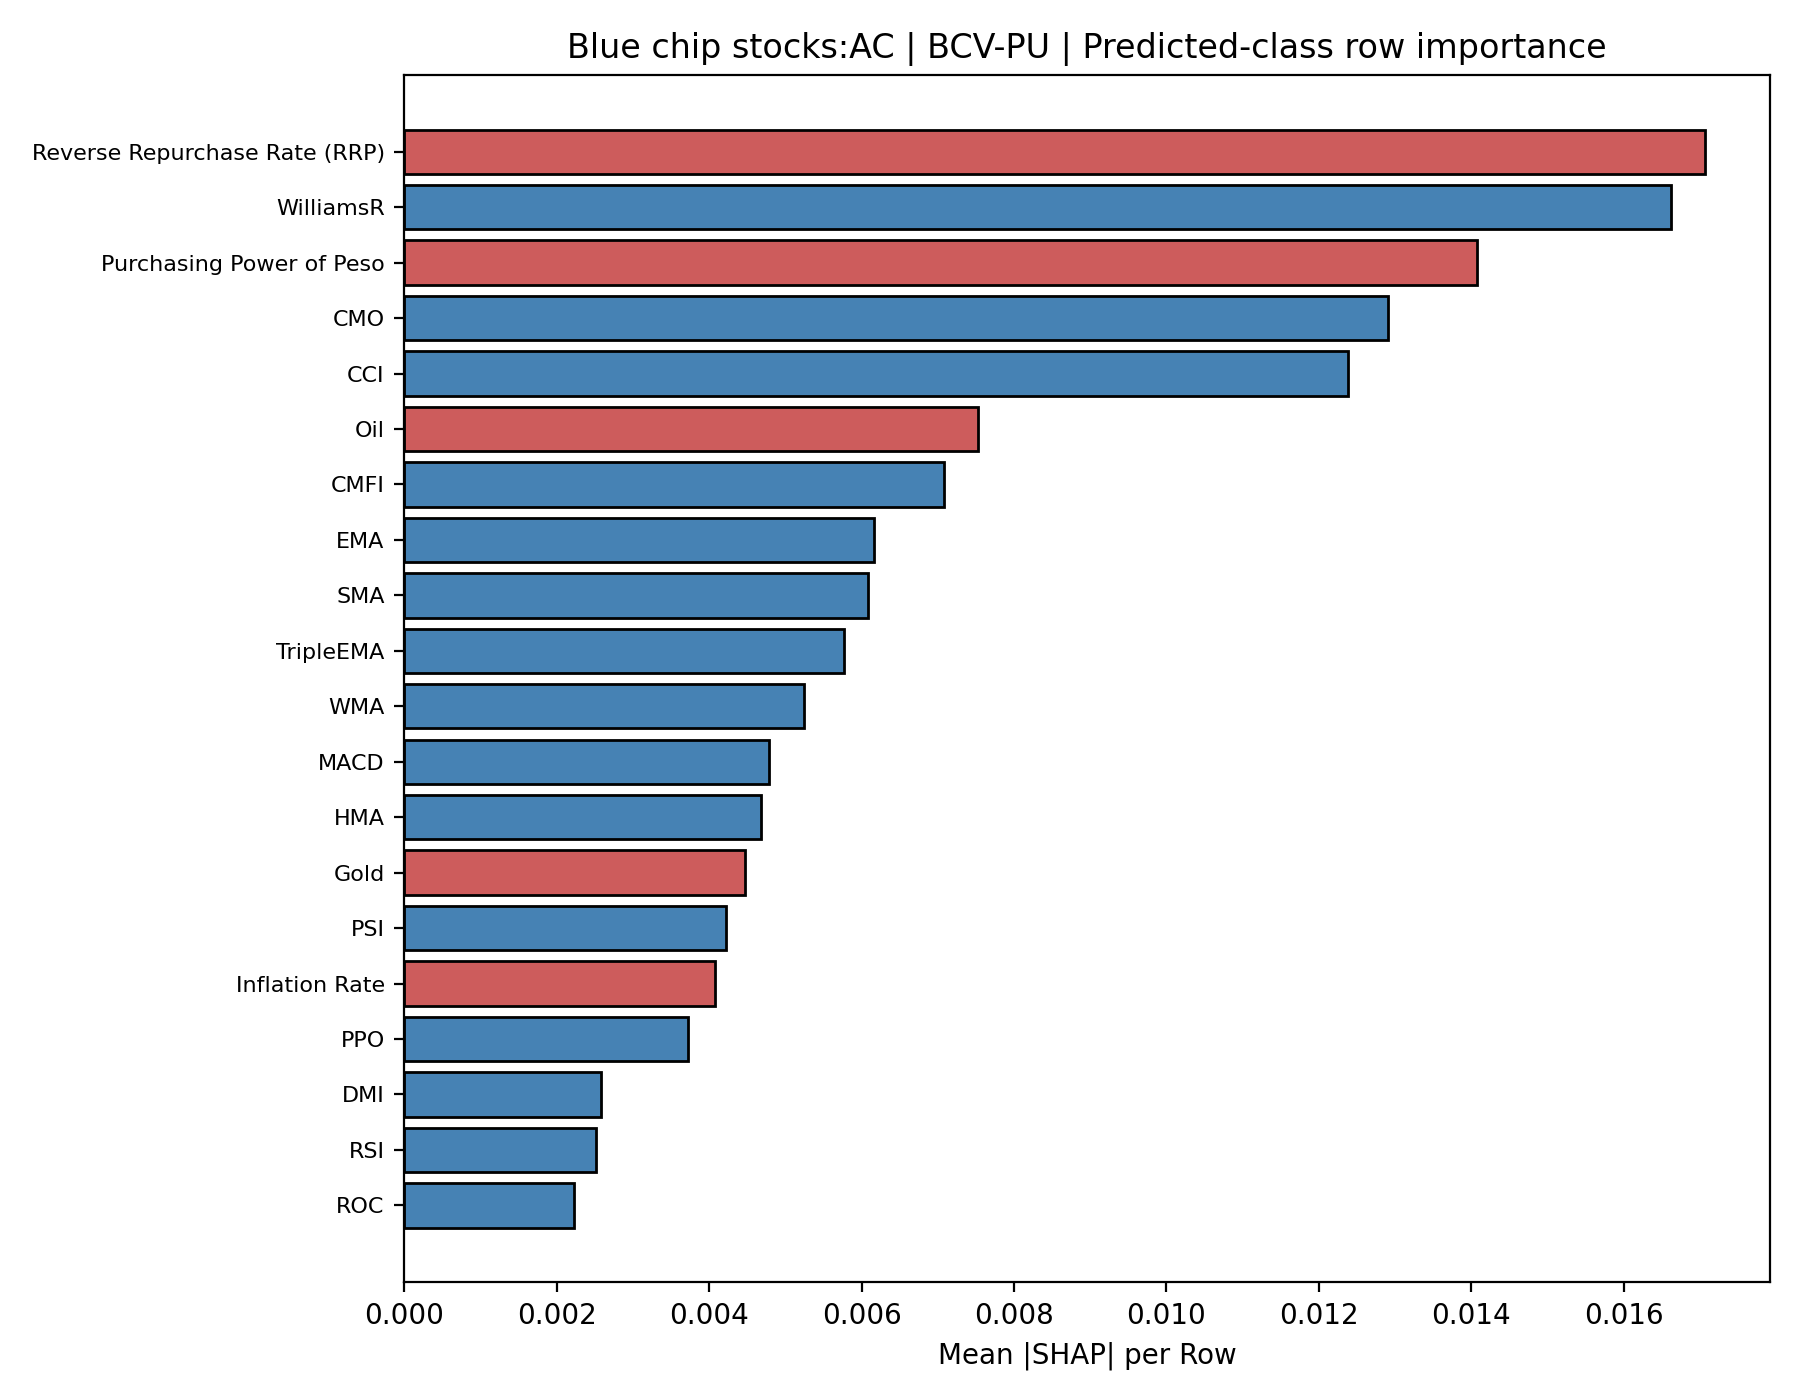
\includegraphics[width=0.32\textwidth]{../figures/AC_PredictedClassRowImportance.png}
	
	\captionof{figure}{Predicted-class SHAP row importance for selected blue-chip stocks under BCV-PU}
	\label{fig:app_shap_bluechip}
\end{center}

\begin{center}
	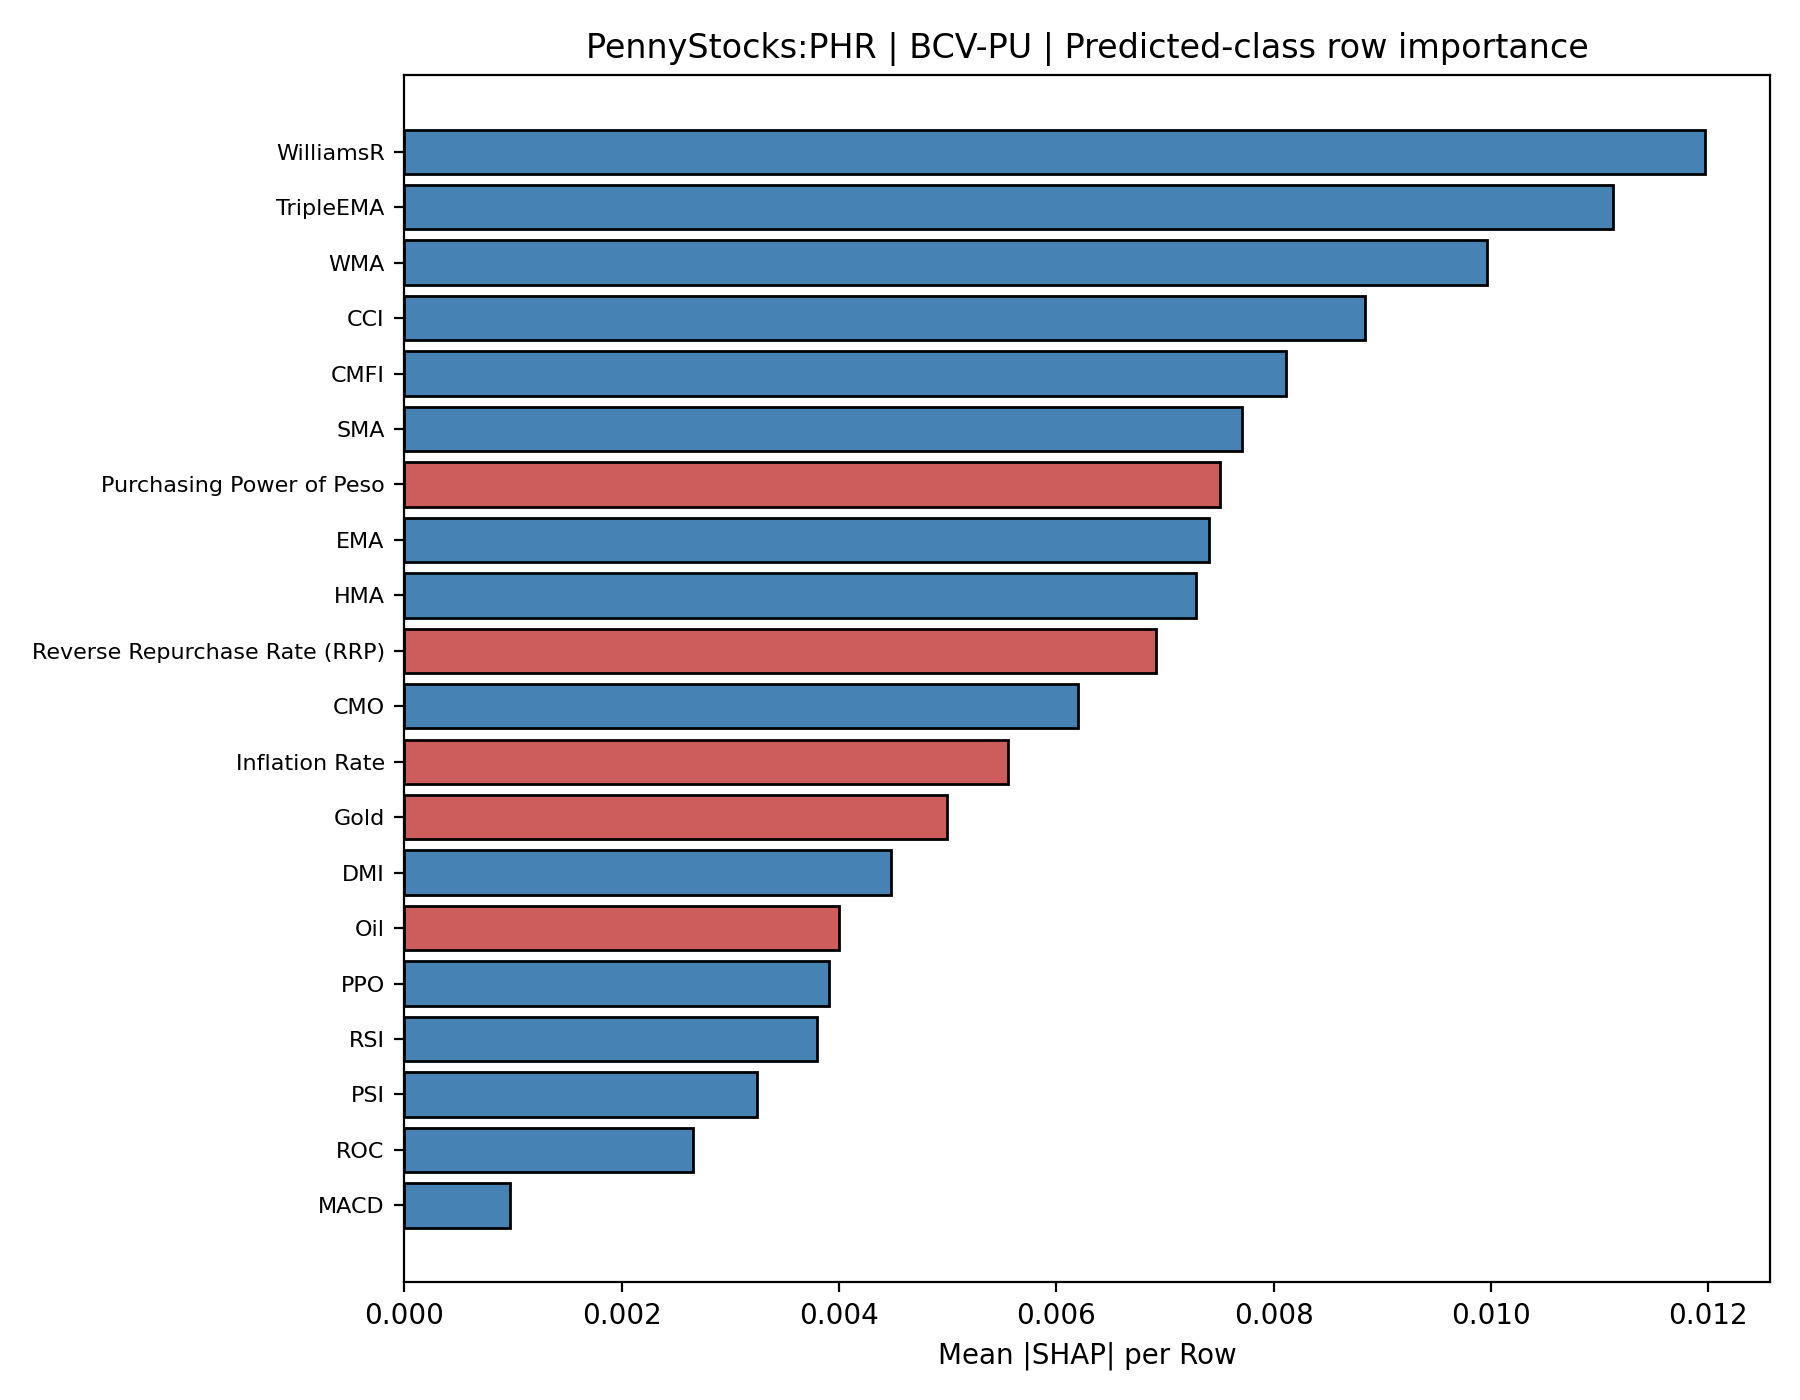
\includegraphics[width=0.32\textwidth]{../figures/PHR_PredictedClassRowImportance.png}
	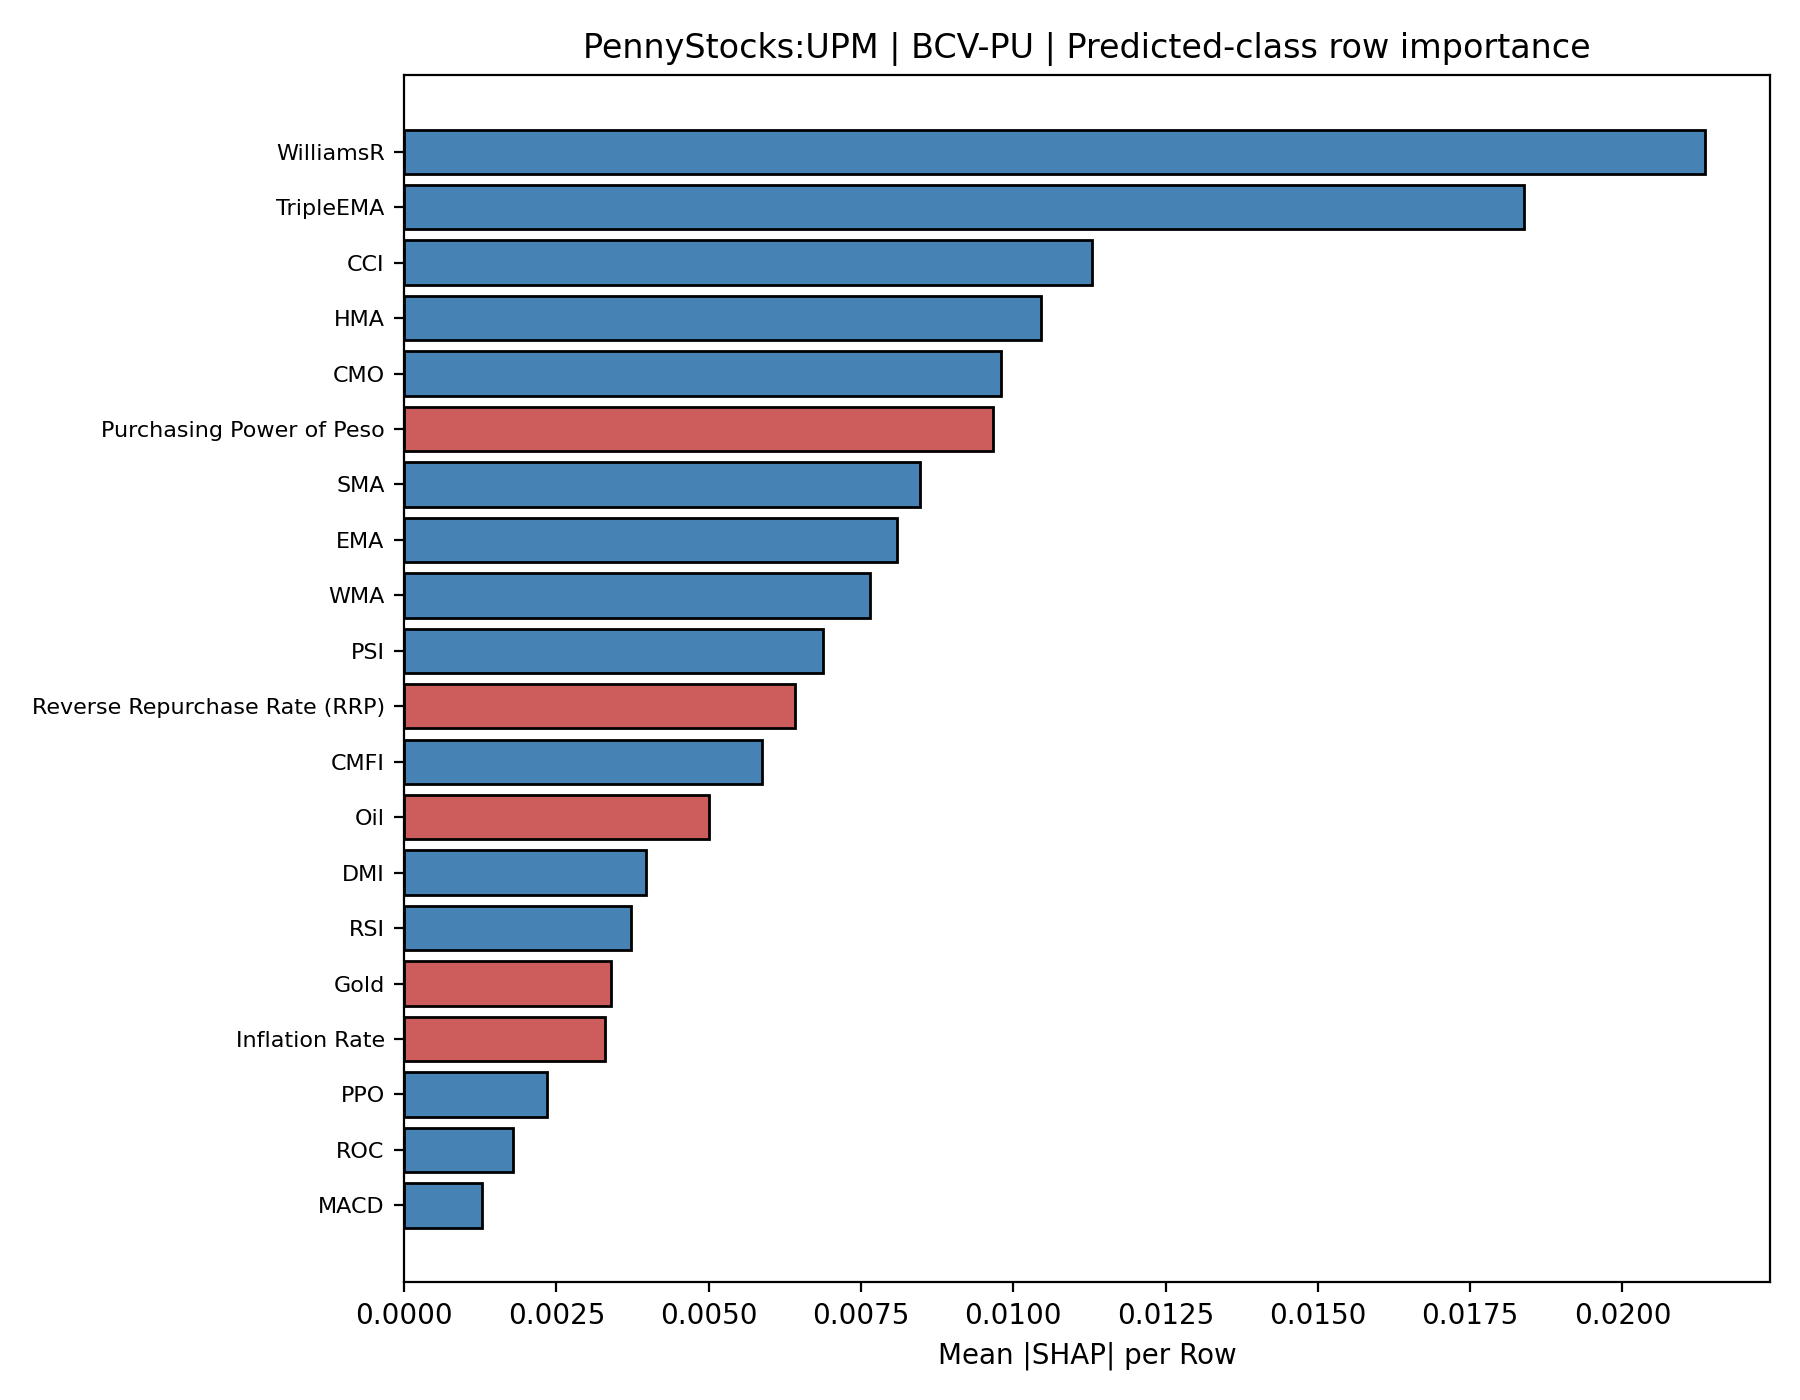
\includegraphics[width=0.32\textwidth]{../figures/UPM_PredictedClassRowImportance.png}
	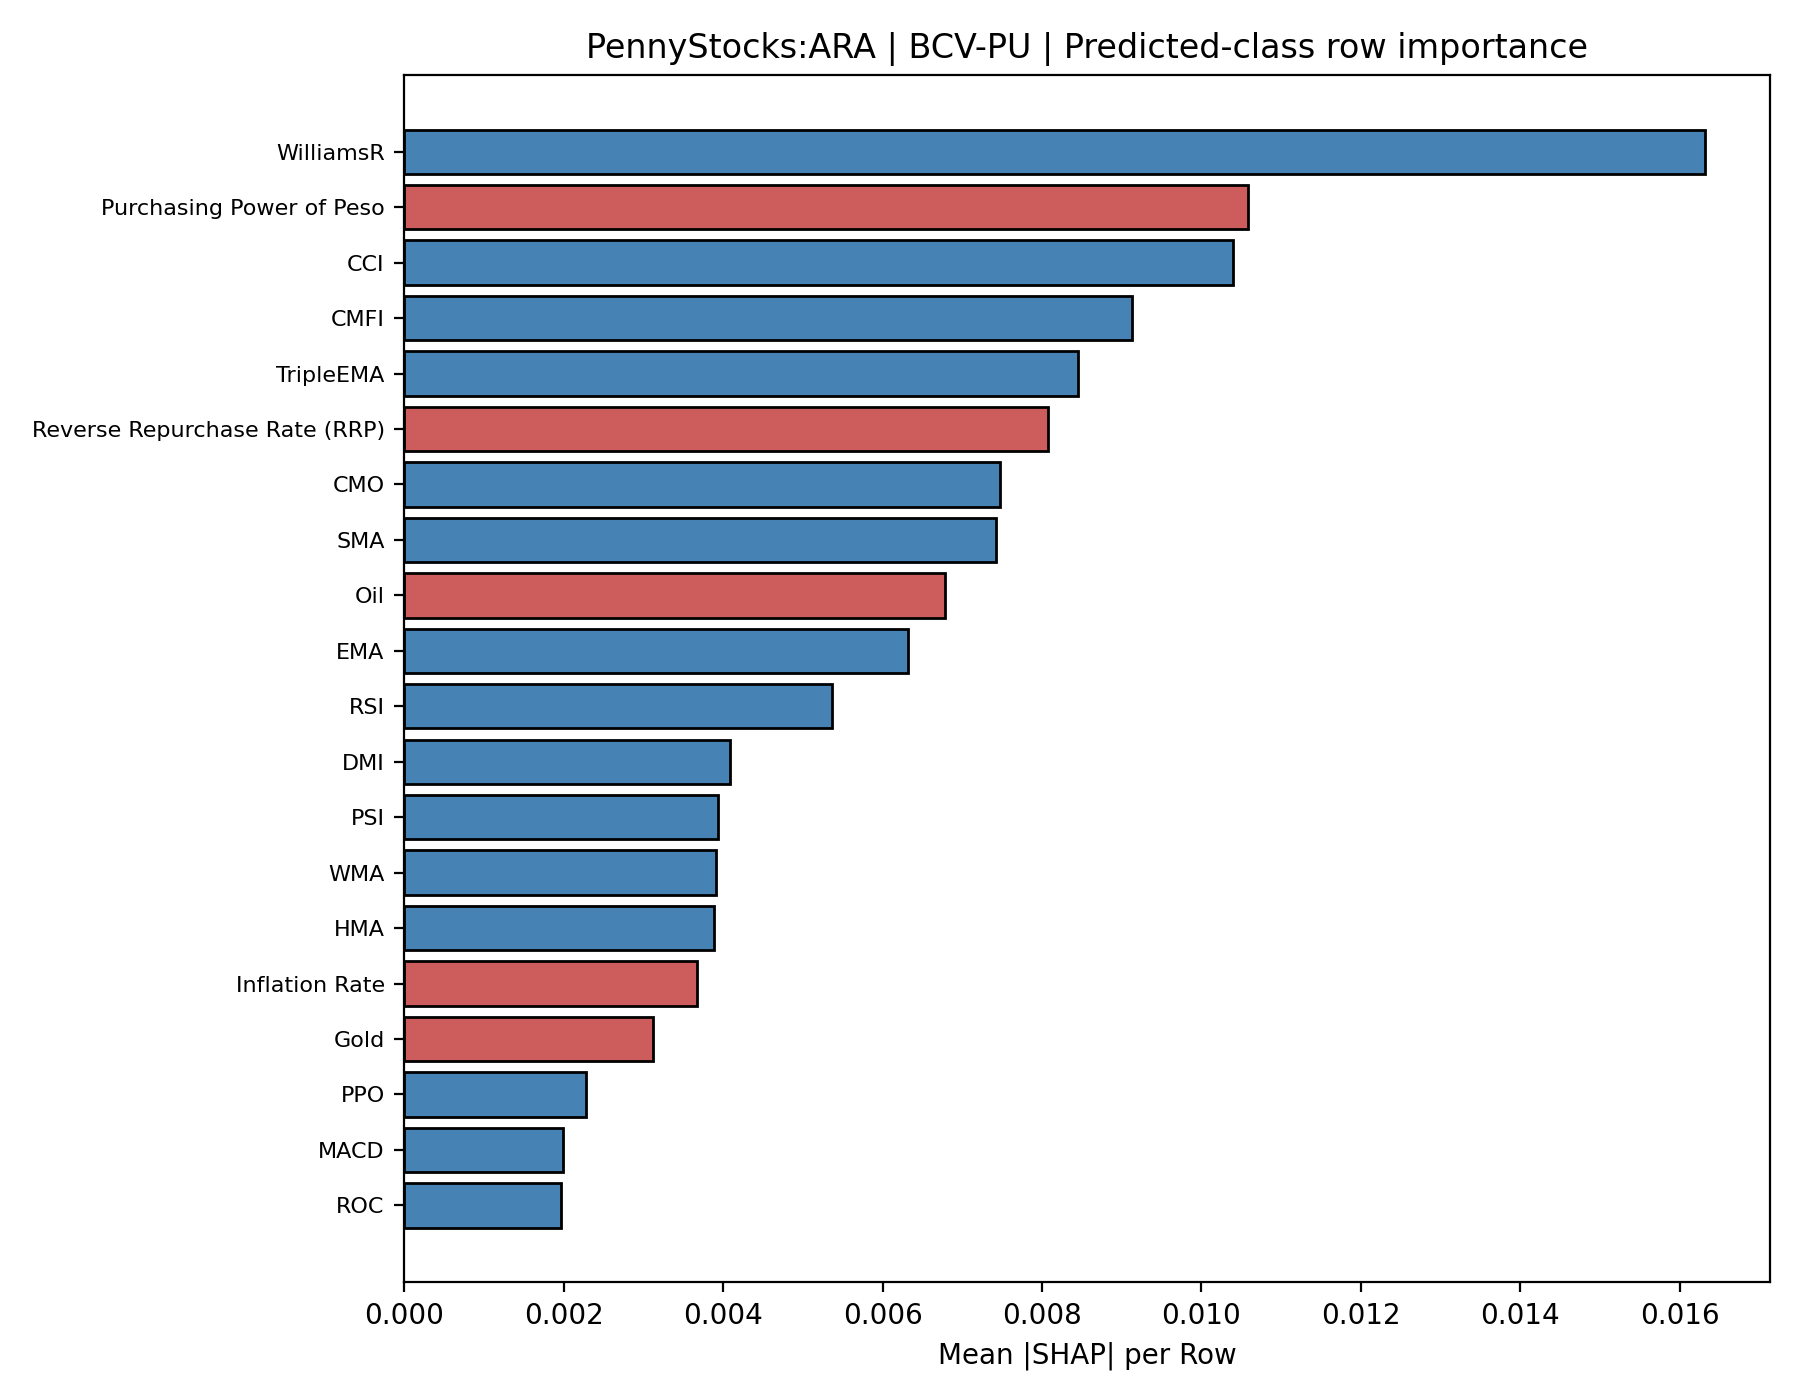
\includegraphics[width=0.32\textwidth]{../figures/ARA_PredictedClassRowImportance.png}
	
	\captionof{figure}{Predicted-class SHAP row importance for selected penny stocks under BCV-PU}
	\label{fig:app_shap_penny}
\end{center}

\begin{center}
	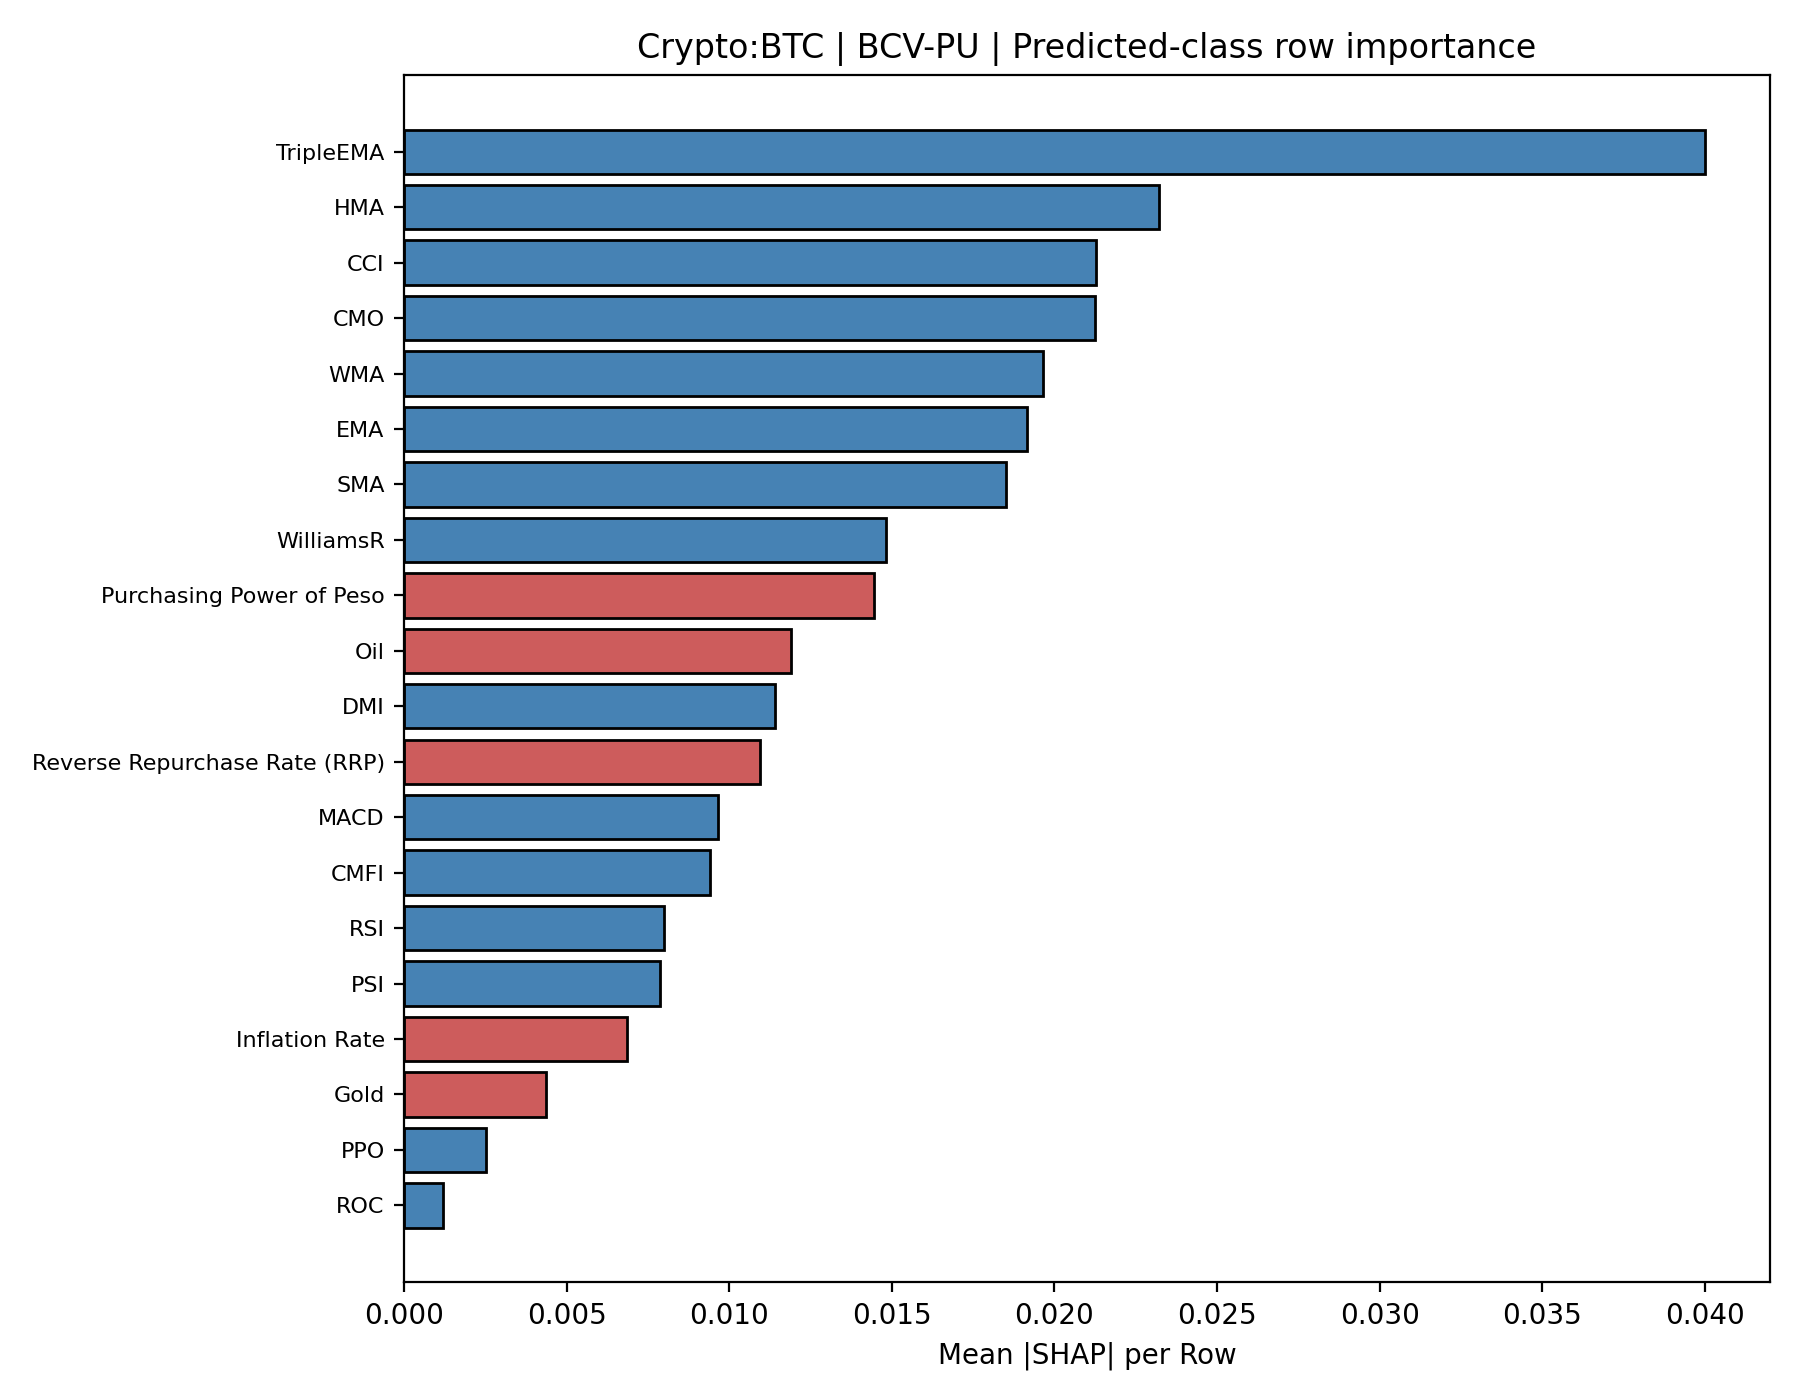
\includegraphics[width=0.32\textwidth]{../figures/BTC_PredictedClassRowImportance.png}
	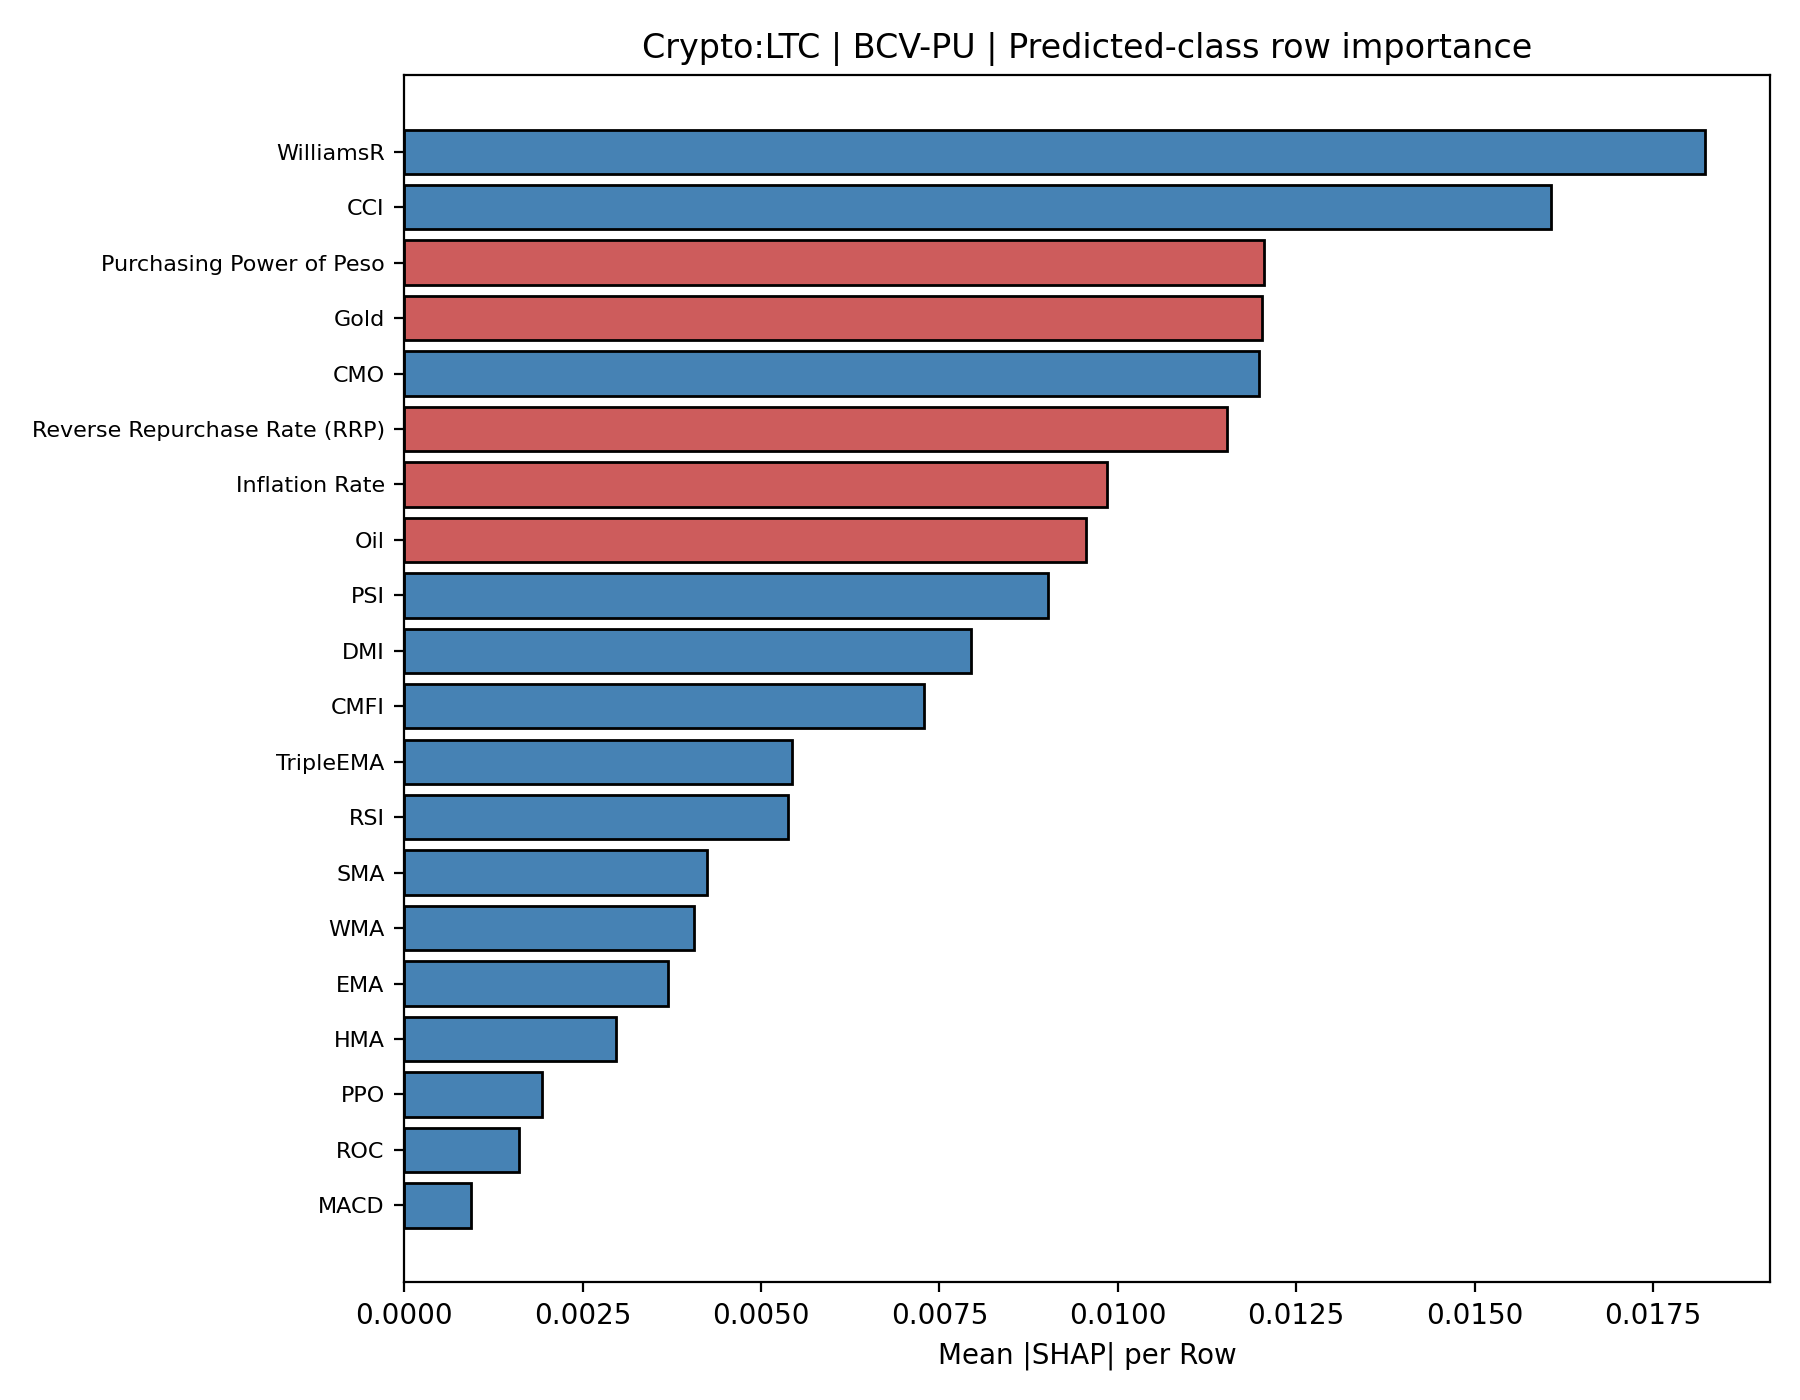
\includegraphics[width=0.32\textwidth]{../figures/LTC_PredictedClassRowImportance.png}
	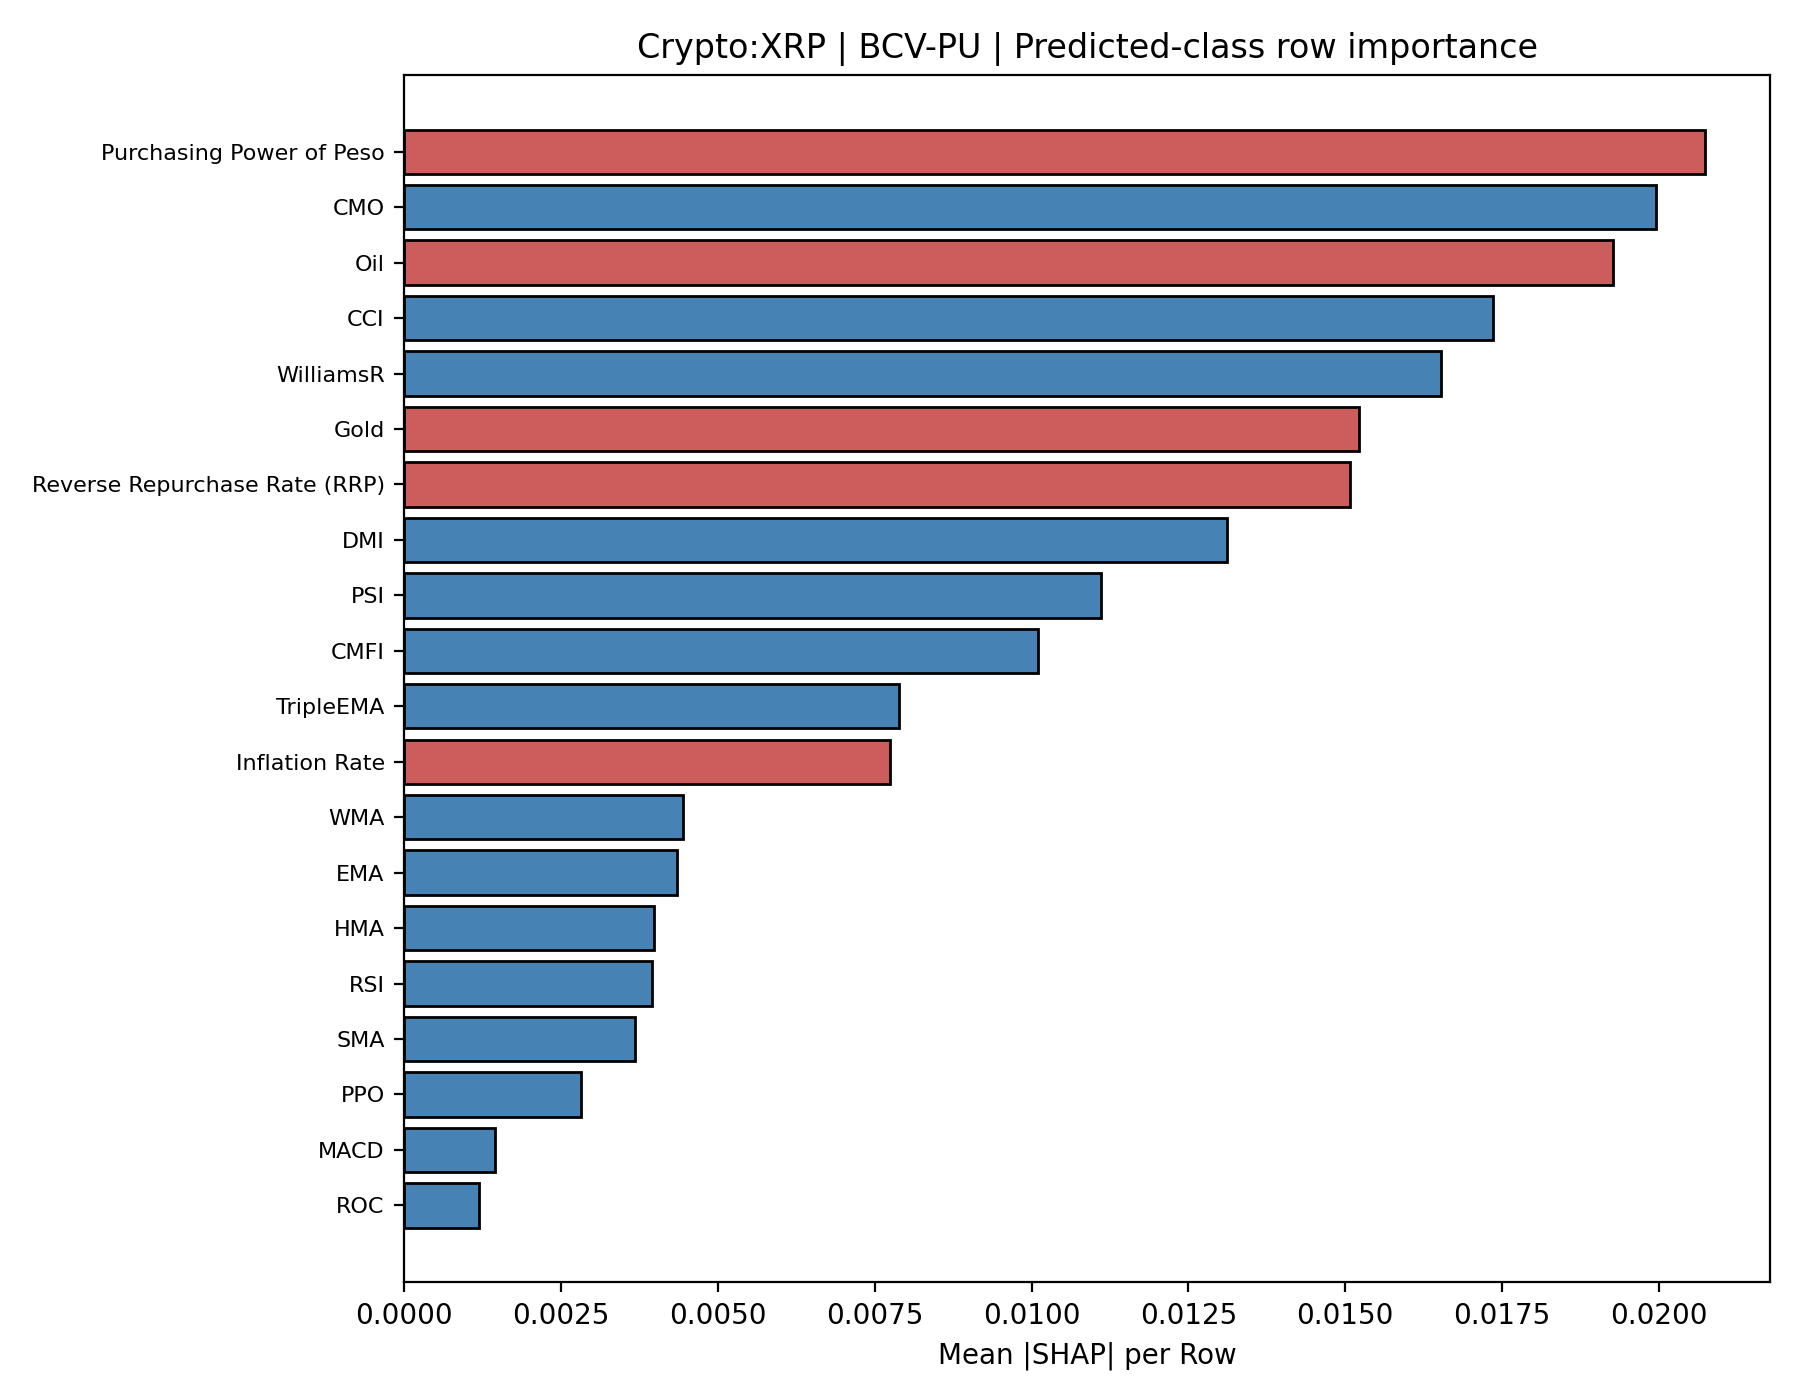
\includegraphics[width=0.32\textwidth]{../figures/XRP_PredictedClassRowImportance.png}
	
	\captionof{figure}{Predicted-class SHAP row importance for selected cryptocurrency assets under BCV-PU}
	\label{fig:app_shap_crypto}
\end{center}

\section{Confusion Matrices}
This section presents the confusion matrices for Blocked Cross-Validation with Partial Undersampling. 

\subsection{Ayala Corporation}

Table~\ref{tab:cm_ac} shows the CNN--TIC and CNN--MIC confusion matrix for Ayala Corporation under Blocked Cross-Validation with Partial Undersampling. Each row represents the true class, while each column represents the class predicted by the model.

\begin{center}
	\scriptsize
	\captionof{table}{Confusion matrix of Ayala Corporation in BCV-PU}
	\label{tab:cm_ac}
	\vspace{0.5em}
		{\renewcommand{\arraystretch}{1.2}
			\resizebox{\textwidth}{!}{%
			\begin{tabular}{llccc}
				\hline
				Model & True Class & Pred Sell & Pred Hold & Pred Buy \\
				\hline
				CNN--TIC & Sell & 26 & 21 & 0 \\
				& Hold & 75 & 361 & 112 \\
				& Buy & 0 & 12 & 37 \\
				\hline
				CNN--MIC & Sell & 30 & 17 & 0 \\
				& Hold & 83 & 377 & 88 \\
				& Buy & 0 & 14 & 35 \\
				\hline
			\end{tabular}
		}
	}
\end{center}

It can be seen that the number of correct CNN--MIC predicts the Hold class, while CNN--TIC does better in the Buy class. It is also noteworthy that there are more Hold to Buy misclassifications in CNN--TIC, which provides further explanation for the difference in their BCV-PU results.

\subsection{Jollibee Foods Corporation}
Table~\ref{tab:cm_jfc} shows the CNN--TIC and CNN--MIC confusion matrix for Jollibee Foods Corporation under Blocked Cross-Validation with Partial Undersampling. Each row represents the true class, while each column represents the class predicted by the model.

\begin{center}
	\centering
	\scriptsize
	\captionof{table}{Jollibee Foods Corporation's Confusion matrix in BCV-PU}
	\label{tab:cm_jfc}
	\renewcommand{\arraystretch}{1.2}
	\resizebox{\textwidth}{!}{%
		\begin{tabular}{llccc}
			\hline
			Model & True Class & Pred Sell & Pred Hold & Pred Buy \\
			\hline
			
			CNN--TIC & Sell & 25 & 23 & 0 \\
			& Hold & 69 & 390 & 93 \\
			& Buy & 0 & 6 & 37 \\
			\hline
			CNN--MIC & Sell & 30 & 18 & 0 \\
			& Hold & 85 & 418 & 49 \\
			& Buy & 0 & 23 & 20 \\
			\hline
		\end{tabular}%
	}
\end{center}

It can be seen that the number of correct CNN--MIC predicts the Hold class, while CNN--TIC performs better in the Buy class. It is also noteworthy that there are more Hold to Buy misclassifications in CNN--TIC, which provides further explanation for the difference in their BCV-PU results.
\subsection{SM Investments Corporation}

Table~\ref{tab:cm_smi} shows the CNN--TIC and CNN--MIC confusion matrix for SM Investments Corporation under Blocked Cross-Validation with Partial Undersampling. Each row represents the true class, while each column represents the class predicted by the model.

\begin{center}
	\centering
	\scriptsize
	\captionof{table}{Confusion matrix of SM Investments Corporation in BCV-PU}
	\label{tab:cm_smi}
	\renewcommand{\arraystretch}{1.2}
	\resizebox{\textwidth}{!}{%
		\begin{tabular}{llccc}
			\hline
			Model & True Class & Pred Sell & Pred Hold & Pred Buy \\
			\hline
			
			CNN--TIC & Sell & 12 & 28 & 0 \\
			& Hold & 17 & 504 & 40 \\
			& Buy & 0 & 21 & 21 \\
			\hline
			CNN--MIC & Sell & 22 & 18 & 0 \\
			& Hold & 50 & 459 & 52 \\
			& Buy & 0 & 15 & 27 \\
			\hline
		\end{tabular}%
	}
\end{center}
It can be seen that CNN--TIC has a higher number of correct predictions in the Hold class, and CNN--MIC has a clearer advantage in the Buy class. It is also noteworthy that CNN--MIC has a higher number of misclassifications from Hold to Buy, which provides further explanation for the difference in their BCV-PU results.



\subsection{Araneta Properties}

The confusion matrix of CNN--TIC and CNN--MIC for Araneta Properties under Blocked Cross-Validation with Partial Undersampling is shown in Table~\ref{tab:cm_ara}. Each row represents the true class, while each column represents the class predicted by the model.

\begin{center}
	\centering
	\scriptsize
	\captionof{table}{Confusion matrix of Araneta Properties in BCV-PU}
	\label{tab:cm_ara}
	\renewcommand{\arraystretch}{1.2}
	\resizebox{\textwidth}{!}{%
		\begin{tabular}{llccc}
			\hline
			Model & True Class & Pred Sell & Pred Hold & Pred Buy \\
			\hline
			
			CNN--TIC & Sell & 18 & 24 & 1 \\
			& Hold & 42 & 260 & 239 \\
			& Buy & 0 & 6 & 40 \\
			\hline
			CNN--MIC & Sell & 11 & 30 & 2 \\
			& Hold & 20 & 230 & 291 \\
			& Buy & 0 & 3 & 43 \\
			\hline
		\end{tabular}%
	}
\end{center}

It can be seen that the number of correct predictions is higher CNN--TIC in the Hold class, and CNN--MIC also has a clearer advantage in the Buy class. It is also noteworthy that there are more misclassifications from Hold to Buy in CNN--MIC, which provides further explanation for the difference in their BCV-PU results.

\subsection{PH Resorts Group}

The confusion matrix of CNN--TIC and CNN--MIC for PH Resorts Group under Blocked Cross-Validation with Partial Undersampling can be seen in Table~\ref{tab:cm_phr}. Each row refers to the true class, while each column refers to the class predicted by the model.

\begin{center}
	\centering
	\scriptsize
	\captionof{table}{Confusion matrix of PH Resorts Group in BCV-PU}
	\label{tab:cm_phr}
	\renewcommand{\arraystretch}{1.2}
	\resizebox{\textwidth}{!}{%
		\begin{tabular}{llccc}
			\hline
			Model & True Class & Pred Sell & Pred Hold & Pred Buy \\
			\hline
			
			CNN--TIC & Sell & 0 & 42 & 0 \\
			& Hold & 0 & 467 & 77 \\
			& Buy & 0 & 40 & 17 \\
			\hline
			CNN--MIC & Sell & 2 & 34 & 6 \\
			& Hold & 3 & 205 & 336 \\
			& Buy & 0 & 1 & 56 \\
			\hline
		\end{tabular}%
	}
\end{center}

It can be seen that the number of correct predictions is higher for CNN--TIC in the Hold class, and CNN--MIC also has a clearer advantage in the Buy class. It is also noteworthy that there are more misclassifications from Hold to Buy in CNN--MIC, which provides further explanation for the difference in their BCV-PU results.\subsection{United Paragon Mining Corporation}

Table~\ref{tab:cm_upm} shows the CNN--TIC and CNN--MIC confusion matrix for United Paragon Mining Corporation under Blocked Cross-Validation with Partial Undersampling. Each row represents the true class, while each column represents the class predicted by the model.

\begin{center}
	\centering
	\scriptsize
	\captionof{table}{Confusion matrix of United Paragon Mining Corporation in BCV-PU}
	\label{tab:cm_upm}
	\renewcommand{\arraystretch}{1.2}
	\resizebox{\textwidth}{!}{%
		\begin{tabular}{llccc}
			\hline
			Model & True Class & Pred Sell & Pred Hold & Pred Buy \\
			\hline
			
			CNN--TIC & Sell & 22 & 4 & 0 \\
			& Hold & 53 & 174 & 22 \\
			& Buy & 0 & 15 & 15 \\
			\hline
			CNN--MIC & Sell & 22 & 4 & 0 \\
			& Hold & 51 & 123 & 75 \\
			& Buy & 0 & 2 & 28 \\
			\hline
		\end{tabular}%
	}
\end{center}

It can be seen that the number of correct predictions is higher CNN--TIC in the Hold class, and CNN--MIC also has a clearer advantage in the Buy class. It is also noteworthy that there are more misclassifications from Hold to Buy in CNN--MIC, which provides further explanation for the difference in their BCV-PU results.

\subsection{Bitcoin}

The confusion matrix of CNN--TIC and CNN--MIC for Bitcoin under Blocked Cross-Validation with Partial Undersampling is shown in Table~\ref{tab:cm_btc}. Each row refers to the true class, while each column refers to the class predicted by the model.

\begin{center}
	\centering
	\scriptsize
	\captionof{table}{Confusion matrix of Bitcoin in BCV-PU}
	\label{tab:cm_btc}
	\renewcommand{\arraystretch}{1.2}
	\resizebox{\textwidth}{!}{%
		\begin{tabular}{llccc}
			\hline
			Model & True Class & Pred Sell & Pred Hold & Pred Buy \\
			\hline
			
			CNN--TIC & Sell & 26 & 38 & 0 \\
			& Hold & 125 & 702 & 12 \\
			& Buy & 11 & 45 & 3 \\
			\hline
			CNN--MIC & Sell & 33 & 31 & 0 \\
			& Hold & 195 & 640 & 4 \\
			& Buy & 23 & 30 & 6 \\
			\hline
		\end{tabular}%
	}
\end{center}

It can be seen that the number of correct predictions is higher CNN--TIC in the Hold class, and CNN--MIC also has a clearer advantage in the Buy class. It is also noteworthy that there are more misclassifications from Hold to Buy in CNN--TIC, which provides further explanation for the difference in their BCV-PU results.

\subsection{Litecoin}

The confusion matrix of CNN--TIC and CNN--MIC for Litecoin under Blocked Cross-Validation with Partial Undersampling is shown in Table~\ref{tab:cm_ltc}. Each row refers to the true class, while each column refers to the class predicted by the model.

\begin{center}
	\centering
	\scriptsize
	\captionof{table}{Confusion matrix of Litecoin in BCV-PU}
	\label{tab:cm_ltc}
	\renewcommand{\arraystretch}{1.2}
	\resizebox{\textwidth}{!}{%
		\begin{tabular}{llccc}
			\hline
			Model & True Class & Pred Sell & Pred Hold & Pred Buy \\
			\hline
			
			CNN--TIC & Sell & 29 & 37 & 0 \\
			& Hold & 58 & 652 & 125 \\
			& Buy & 0 & 12 & 49 \\
			\hline
			CNN--MIC & Sell & 20 & 46 & 0 \\
			& Hold & 45 & 694 & 96 \\
			& Buy & 0 & 17 & 44 \\
			\hline
		\end{tabular}%
	}
\end{center}
It can be seen that CNN--MIC has a higher number of correct predictions for the Hold class, while CNN--TIC has a better performance for the Buy class. It is also noteworthy that CNN--TIC has a higher number of misclassifications from Hold to Buy, which further explains the difference in their BCV-PU results.

\subsection{XRP}

The confusion matrix of CNN--TIC and CNN--MIC for XRP under Blocked Cross-Validation with Partial Undersampling is shown in Table~\ref{tab:cm_xrp}. Each row represents the true class, while each column represents the class predicted by the model.

\begin{center}
	\centering
	\scriptsize
	\captionof{table}{XRP Confusion matrix in BCV-PU}
	\label{tab:cm_xrp}
	\renewcommand{\arraystretch}{1.2}
	\resizebox{\textwidth}{!}{%
		\begin{tabular}{llccc}
			\hline
			Model & True Class & Pred Sell & Pred Hold & Pred Buy \\
			\hline
			
			CNN--TIC & Sell & 59 & 5 & 0 \\
			& Hold & 289 & 477 & 72 \\
			& Buy & 11 & 21 & 27 \\
			\hline
			CNN--MIC & Sell & 56 & 8 & 0 \\
			& Hold & 330 & 486 & 22 \\
			& Buy & 14 & 39 & 6 \\
			\hline
		\end{tabular}%
	}
\end{center}

It can be seen that the number of correct predictions is higher CNN--MIC performs better in the Hold class, while CNN--TIC performs better in the Buy class. It is also noteworthy that there are more misclassifications from Hold to Buy in CNN--TIC, which further explains the difference in their BCV-PU results.